En esta etapa, se lleva a cabo la implementación del diseño del proceso ETL previamente definido, utilizando las herramientas seleccionadas. Se desarrollan los flujos de extracción, transformación y carga de los datos según lo establecido en el diseño.

Una vez implementado, se procede a realizar pruebas exhaustivas para garantizar el correcto funcionamiento del proceso. Estas pruebas incluyen la verificación de la extracción de datos de las fuentes, la correcta aplicación de las transformaciones definidas y la carga exitosa de los datos en el destino final.

El objetivo de las pruebas es asegurar que el proceso ETL cumpla con los requisitos establecidos y que los resultados obtenidos sean los esperados. Esto implica validar la integridad y coherencia de los datos transformados, así como verificar el rendimiento y la escalabilidad del proceso.

En caso de encontrar inconvenientes o desviaciones durante las pruebas, se realizan los ajustes necesarios en el diseño o en la configuración de las herramientas utilizadas. Es fundamental realizar iteraciones y pruebas adicionales hasta obtener resultados consistentes y satisfactorios.

Como primer paso en la construcción del proceso ETL, se importan las bibliotecas pandas y numpy. Luego se le da nombre a las columnas, ya que el contenido del archivo csv solo trae los datos. Una vez nombradas las columnas se ordenan para un entendimiento más facil del conjunto de datos, quedando de la siguiente manera respectivamente: rut, fecha, metodo, canal.

Ahora se comprueba la existencia de valores nulos en el dataframe, resultando lo siguiente:

\begin{figure}[H]
    \begin{minipage}[t]{0.8\textwidth}
        \caption{Valores nulos en el conjunto de datos.}
        \label{valoresNulos}        
    \end{minipage}

    \vspace{10pt}

    \centering
    \begin{minipage}[b]{0.4\textwidth}
        \centering
        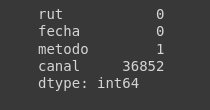
\includegraphics[width=\textwidth]{img/valores-nulos.png}        
    \end{minipage}

    \begin{minipage}[t]{0.9\textwidth}
        Fuente: Elaboración propia.
    \end{minipage}
\end{figure}

Como se puede ver en la imagen anterior solamente los campos 'metodo' y 'canal' poseen valores nulos, de hecho, el primero solo cuenta con un valor nulo. La columna 'canal' cuenta con 36852 valores nulos. Luego de eliminar los valores nulos se pasa a eliminar las filas que contengan métodos inconsistentes o irrelevantes, que son:
\begin{itemize}
    \item reCaptcha()
    \item clientes/surveys
    \item clientes/cuentas/validar-cuenta-corriente
    \item clientes/cuentas/cuentas-bancarias
    \item clientes/cuentas/cuentas-bancarias?rut=******** 
    \item clientes/cuentas/cuentas-bancarias?rut=********
    \item clientes/cuentas/cuentas-bancarias?rut=*********
    \item clientes/cuentas/cuentas-bancarias?rut=*********
    \item clientes/cuentas/cuentas-bancarias?rut=*********
    \item clientes/cuentas/cuentas-bancarias?rut=********
    \item clientes/cuentas/cuentas-bancarias?rut=*********
    \item clientes/cuentas/cuentas-bancarias?rut=*********
    \item clientes/cuentas/APV/solicitud/giros?rut=*********\&account=APV
    \item clientes/cuentas/cuentas-bancarias?rut=*********
\end{itemize}

El método reCaptcha() de Google valida la autenticidad de usuarios frente a bots, pero su utilidad se limita a la seguridad en línea. No ofrece información relevante para predecir el comportamiento de los usuarios en la plataforma, siendo necesario recurrir a los otros datos para comprender mejor sus acciones y patrones de uso.